\newpage
\section{Kurzanleitung}
\label{sec:Kurzanleitung}
% ----------------------
\url{https://www.th-rosenheim.de/international/incoming-students/informationen-fuer-austauschstudierende/studium-in-rosenheim/}
Dies ist eine Kurzanleitung für den Einstieg die jedoch ausreichend ist um die grundlegenden Funktionen der Vorlage zu verstehen.
\par
Beispiele zur Anwendung der Vorlage sind in der Datei \textbf{Anwendungsbeispiele.tex} im Ordner \textbf{01-Content/SampleFiles} enthalten.
Generell ist auch die Hilfe von Overleaf sehr zu empfehlen, da hier sehr viele Anwendungsbeispiele mit kleinen lauffähigen Quellcodes enthalten sind.
%
\subsection{Wahl des Dokumententyps}
Dies ist eine allgemeine Vorlage für das \ac{LaSM} für folgende Dokumententypen:
\begin{description}
    \item[TechnicalReport.cls] Umfangreicher Bericht, z.B. Forschungsbericht
    \item[Memo.cls] Formlose Notizen
    \item[Minutes.cls] Protokoll
    \item[Thesis.cls] Abschlussarbeiten
    \item[Paper.cls] Kurzaufsatz
\end{description}
\textbf{Eine (!)} der fünf Dokumentenklassen kann in der Datei \textbf{LaSM-Master.tex} unter
\begin{lstlisting}[language=tex]
% ==================================================
%       C H O O S E     D O C U M E N T C L A S S (only 1)
% ==================================================    
\end{lstlisting}
ausgewählt werden. 
Dabei muss die gewünschte Klasse die einzige der vorhandenen Klassen sein, die nicht auskommentiert ist.
Soll zum Beispiel die Klasse Thesis.cls geladen werden:
\begin{lstlisting}[language=tex]
% \documentclass{\CLSPath TechnicalReport}
% \documentclass{\CLSPath Memo}
% \documentclass{\CLSPath Minutes}
 \ documentclass{\CLSPath Thesis}
% \documentclass{\CLSPath Paper}
\end{lstlisting}
Die Dokumentenklassen unterscheiden sich in ihrem Aufbau und Erscheinungsbild. 
So wird der Bericht standardmäßig zweiseitig angelegt mit einer Reihe von Verzeichnissen im Gegensatz zu einer Notiz.
\par 
Unter 
\begin{lstlisting}[language=tex]
% ==================================================
%       T I T L E ,  N A M E S ,  K E Y W O R D S
% ================================================== 
%
% General Commands
% --------------------------------------------------
\end{lstlisting}
werden für alle Klassen Angaben zu Titel etc. gemacht.
Diese Angaben werden auch in die Metadaten des fertigen pdf Dokuments geschrieben.
\par
In den Klassen \textit{Technical Report} und \textit{Thesis} sind zusätzliche Angaben unter
\begin{lstlisting}[language=tex]
% Specific for   T E C H N I C A L   R E P O R T
% --------------------------------------------------
\end{lstlisting}
bzw.
\begin{lstlisting}[language=tex]
% Specific for   T H E S I S
% --------------------------------------------------
\end{lstlisting}
zu machen.
%
\subsection{Das Frontmatter}
Das Frontmatter (deutsch: \textit{Titelei}) sind die Seiten bevor das eigentliche Dokument beginnt.
Diese Seiten sind mit römischen Seitenzahlen versehen.
Für die Dokumentenklassen \textit{Technical Report} und \textit{Thesis} werden im Frontmatter folgende Seiten hinzugefügt:
\begin{itemize}
    \item \textbf{Titelseite} (wird automatisch erstellt)
    \item \textbf{Erklärung} (wird automatisch erstellt)
    \begin{itemize}
        \item nur bei Dokumentenklasse \textit{Thesis}
        \item Text kann bei Bedarf in \textbf{13-Frontmatter/Erklaerung} abgeändert werden
    \end{itemize}
    \item \textbf{Kurzfassung} (Text in \textbf{13-Frontmatter/Abstract} schreiben)
    \item \textbf{Danksagung} (Text in \textbf{13-Frontmatter/Acknowledgements} schreiben) 
    \item \textbf{Inhaltsverzeichnis} (wird automatisch erstellt)
    \item \textbf{Abbildungsverzeichnis} (wird automatisch erstellt)
    \item \textbf{Tabellenverzeichnis} (wird automatisch erstellt)
    \item \textbf{Symbolverzeichnis} (wird automatisch erstellt, siehe auch \ref{sec:Beispiele_SymboleAbk_Symbole})
    \item \textbf{Abkürzungsverzeichnis} (wird automatisch erstellt, siehe auch \ref{sec:Beispiele_SymboleAbk_Abk})
\end{itemize}
%
\subsection{Inhalt erzeugen}
In dem Ordner \textbf{01-Content} muss eine Datei angelegt werden und dann in der \textbf{LaSM-Master.tex} unter 
\begin{lstlisting}[language=tex]
% ==================================================
%       Y O U R   C O N T E N T 
% ==================================================   
\end{lstlisting}
eingefügt werden.
Hierfür folgende Codezeile verwenden:
\begin{lstlisting}[language=tex]
\import{01-Content/}{<Dateiname>}
\end{lstlisting}
Bei umfangreichen Berichten ist es empfehlenswert je Hauptkapitel oder ggf. auch für jeden Abschnitt eine Datei anzulegen statt einer Datei für den gesamten Inhalt.

\subsubsection{Besonderheit: Anhang}
In den Klassen \textit{Technical Report} und \textit{Thesis} kann optional ein Anhang unter
\begin{lstlisting}[language=tex]
% ==================================================
%       Y O U R   A P P E N D I X
% ==================================================   
\end{lstlisting}
eingefügt werden.
Abschnitte des Anhanges werden analog unter Verwendung von
\begin{lstlisting}[language=tex]
\import{01-Content/}{<Dateiname>}
\end{lstlisting}
eingefügt.
%
\subsection{Grafiken einfügen}
In dem Ordner \textbf{02-Figures} sollten alle Bilder abgelegt werden.
Ein Bild kann im einfachsten Fall wie in Abbildung \ref{fig:my_exampleFigure} folgt eingefügt werden.
\begin{figure}
    \centering % zentrieren des Bildes
    \includegraphics{\GraficPath Logo-THRo}
    \caption{Beispiel zum Einfügen eines Bildes} % Abbildungsbeschriftung
    \label{fig:my_exampleFigure}
\end{figure}

\subsection{!!! Praktische Hinweise und Empfehlungen !!!}
%
Diese Hinweise und Empfehlungen sind hilfreich und ersparen evtl. viel Zeit wenn man sie von Anfang an befolgt. \textbf{Unbedingt lesen!}
%
\begin{itemize}
	\item \textbf{Das Dokument in kleinere *.tex Dateien aufteilen} (z.B. für jedes Kapitel oder sogar jeden Abschnitt eine eigene Datei). 
	Das hat den Vorteil die Übersicht zu behalten und bei Bedarf nur Teile des Dokumentes zu übersetzen um Übersetzungsziet während der Schreibphase zu minimieren.
	\item Im Code \textbf{nach jedem Satz eine neue Codezeile beginnen}.
	Dadurch wird die Fehlersuche optimiert und man kann leichter vom pdf in den Code und adersrum springen.
	\item \textbf{Keine Leerzeilen im Code}. Wenn Leerzeilen zur Übersicht eingefügt werden, dann als auskommentierte Zeilen.
	\item \textbf{Absätze bewusst} mit dem Befehl
	\begin{lstlisting}[language=tex]
\par\end{lstlisting}
    \textbf{setzen}.
	\item Nach Möglichkeit \textbf{keine Änderungen in den *.sty Files} vornehmen\footnote{Ausnahmen: Commands.sty und Hyphenation.sty}, es sei denn man weiß wirklich was man macht.
	Die Vorlage funktioniert. Es reicht wenn man in \textbf{LaSM-Master.tex} die Dokumentenklasse wählt und die nötigen Informationen zum Titel etc. macht.
	Der Inhalt der Arbeit kommt dann in eigene *.tex Dateien die im Folder \textbf{01-Content/} abgelegt werden und in \textbf{LaSM-Master.tex} mit dem Befehl
	%
	\begin{lstlisting}[language=tex]
\import{\ContentPath}{<Dateiname>}\end{lstlisting}
	%	
	zum Dokument hinzugefügt werden.
	\item \textbf{Symbole aus} dem vorhandenen \textbf{Symbolverzeichnis} \textbf{Symbols.tex} im Ordner \textbf{13-Frontmatter} \textbf{verwenden} (siehe Abschnitt \ref{sec:Beispiele_SymboleAbk_Symbole}). 
	Hier sind bereits viele Symbole korrekt nach \citeauthor{DINENISO800004:202001} oder anderen Normen hinterlegt.
	\item In gleicher Weise können \textbf{Abkürzungen} in der Datei \textbf{Abbreviations.tex} im Ordner \textbf{13-Frontmatter} festgelegt und im Dokument verwendet werden (siehe Abschnitt \ref{sec:Beispiele_SymboleAbk_Abk}).
	\item \textbf{Zahlen und Einheiten} mit dem Paket siunitx setzen (siehe Abschnitt \ref{sec:Beispiele_EinheitenZahlen}).
	\item Für \textbf{Abbildungs- und Tabellenbeschriftung} die Möglichkeit nutzen, eine lange Version im Text und eine kurze Version für das Verzeichnis zu setzen:
	\begin{lstlisting}[language=tex]
\caption[<Kurzbeschriftung>]{<Ausfuehrliche Beschriftung>}\end{lstlisting}
    \item \textbf{Die Labels für Querverweise mit einem Präfix versehen}, so behält man bei vielen Verweisen den Überblick. Z.B. \textit{fig:<name>, sec:<name>, tab:<name> und eq:<name>} für die vier Gruppen Figures, Kapitel/Abschnitte, Tabellen und Gleichungen.
    Für die Labels von Kapiteln und Abschnitten hat es sich als praktisch erwiesen, übergeordnete Abschnitte im Label mitzuziehen. So bekommt ein Kapitel z.B. das Label \textit{sec:Kapitel1}, der erste Abschnitt (section) würde dann z.B. \textit{sec:Kapitel1\_Abschn1} bekommen, die darunter liegende subsection \textit{sec:Kapitel1\_Abschn1\_XYZ} usw.\\
    \textbf{Achtung: Keine Umlaute oder Sonderzeichen in Labels für Querverweise verwenden!}
	\item \textbf{Während des Schreibens noch keine Gedanken über die Position von Tabellen und Abbildungen machen.}
	Latex setzt diese in der Regel oben auf der Seite an der Stelle wo es gut passt.
	Darauf kann zwar Einfluss genommen werden, das macht aber erst Sinn wen der Text fertig steht.
	\item \textbf{Bilder und Fotos} die als Pixelgrafiken einfügt werden \textbf{sollten} in der Größe \textbf{auf die benötigte Druckgröße} mit einer Auflösung von mindestens 300dpi \textbf{reduziert werden}.
	Werden Fotos mit der Auflösung von mehreren Megapixel eingefügt wird das pdf sehr groß und die Übersetzung des Quellcodes zum pdf dauert sehr lange.
	\item \textbf{Tabellen} mit dem tool unter \url{http://www.tablesgenerator.com/} erstellen. Dabei nicht den \textit{Default table style} sondern den \textbf{\textit{Booktabs table style}} verwenden. Das benötigte Paket \textit{booktabs} ist in der Vorlage bereits enthalten.
	\item \textbf{Verwendung der todo-notes} (Siehe Abschnitt \ref{sec:ToDoNotes})
	\item \textbf{Trennregeln} für unbekannte Wörter konnen in der Datei \textbf{Hyphenation.sty} im Ordner \textbf{12-Styles-Packages} definiert werden.
	\item Für immer \textbf{wiederkehrende Begriffe} können in der Datei \textbf{Commands.sty} im Ordner \textbf{12-Styles-Packages} Kurzbefehle und Schreibweisen festgelegt werden.
\end{itemize}
%
%
%
\newpage
\section{Nutzung von Overleaf}
% ----------------------
%
Overleaf kann einfach ohne Installation im Browser verwendet werden.
Besonders zu empfehlen ist die Hilfe von Overleaf.
Hier ist neben der Bedienung von Overleaf vor allem eine grundlegende Einführung in \LaTeX beschrieben.
%
\subsection{Oberfläche}
In Abbildung \ref{fig:Overleaf} ist die Oberfläche von Overleaf im Browser dargestellt.
%
\begin{figure}[bht]
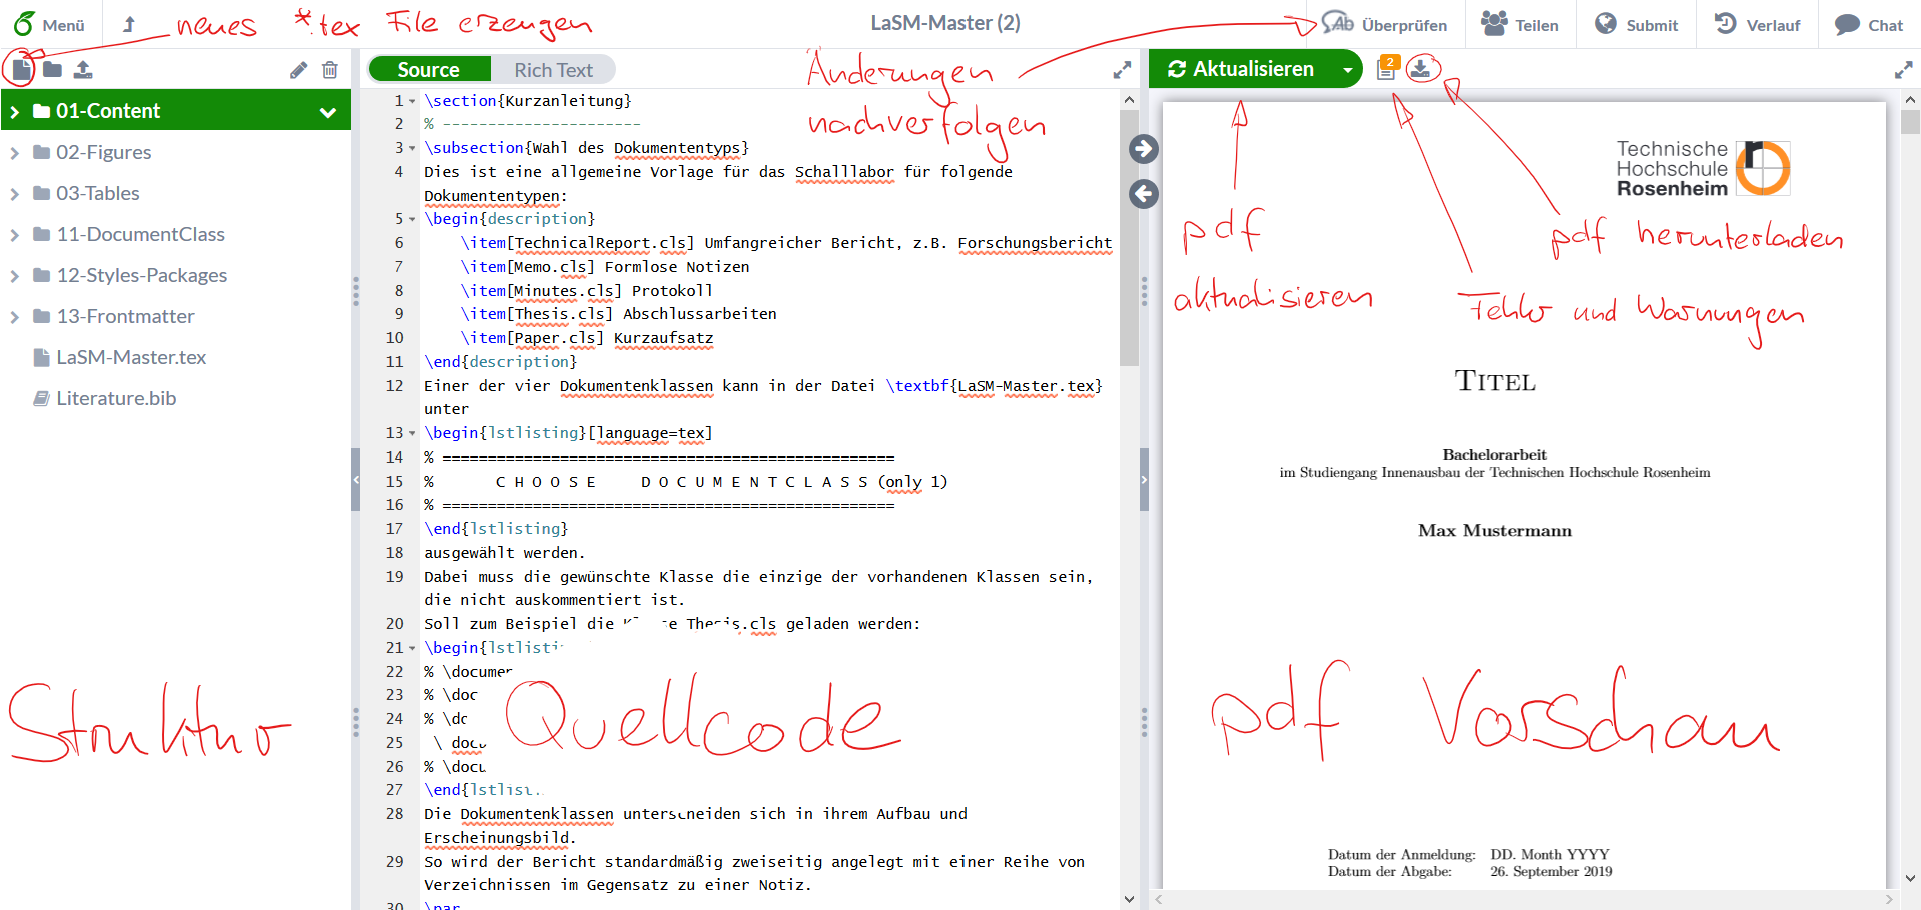
\includegraphics[width=\linewidth]{\GraficPath SampleFigs/Overleaf}
\caption{Oberfläche Overleaf im Webbrowser}
\label{fig:Overleaf}
\end{figure}
%
\subsection{Tastenbefehle}
Folgende Tastenbefehle sind in Overleaf nützlich. Eine ausführliche Liste ist auch unter Menü/Show Hotkeys zu finden.
\par
%
\begin{tabular}{ll}
Strg+Enter                  & Compile (Übersetzen)\\
Strg+Shift+7 bzw. Strg+/    & Kommentieren\\
Strg+B                      & Markierten Text fett setzen\\
Strg+I                      & Markierten Text kursiv setzen\\
Strg+F                      & Suchen und ersetzen
\end{tabular}
%
\subsection{Speichern}
Zwischenspeichern wie in Word ist nicht notwendig.
Über die \textit{History} rechts oben in der Oberfläche können frühere Zustände vom Dokument wiederhergestellt werden.
\par
Evtl. bietet es sich an das ganze Projekt auf GitHub, Git oder auch Dropbox zu sychronisieren.
Das ist unter Menü - Sync möglich. 
Für diese Funktion ist allerdings die Pro-Version erforderlich.
Hierfür Fabian Schöpfer ansprechen, der verwaltet den Account und kann die Pro-Version freischalten.
\par
Alternativ kann das gesamte Projekt als *.zip Datei heruntergeladen werden.
Dies geht unter Menü - Download - Source.